% Asset ID: A22MomentsTikZ-003
% Source: MechYr2 Chapter 4 Moments, page 12; Rigid Bodies transcript section 2.
% Related lesson section: Core Theory 2; Core Theory 3.
% Purpose: Rigid-body equilibrium summary.

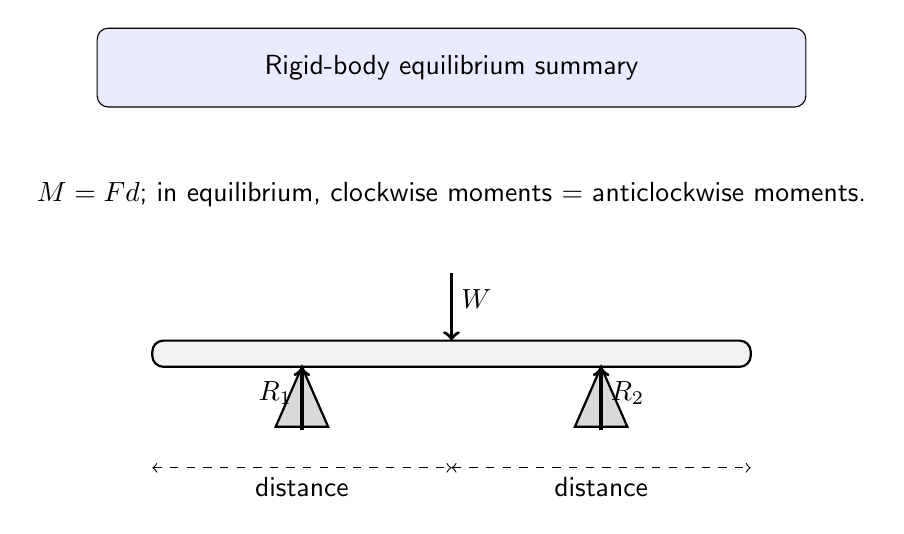
\begin{tikzpicture}[scale=0.95, every node/.style={font=\sffamily}]
  \node[draw, rounded corners, fill=blue!8, align=center, minimum width=9cm, minimum height=1cm] at (4,4) {Rigid-body equilibrium summary};
  \draw[fill=gray!10, thick, rounded corners] (0,0) rectangle (8,0.35);
  \draw[fill=gray!30, thick] (2,0) -- (1.65,-0.8) -- (2.35,-0.8) -- cycle;
  \draw[fill=gray!30, thick] (6,0) -- (5.65,-0.8) -- (6.35,-0.8) -- cycle;
  \draw[->, very thick] (2,-0.85) -- (2,0);
  \node[left] at (2,-0.35) {$R_1$};
  \draw[->, very thick] (6,-0.85) -- (6,0);
  \node[right] at (6,-0.35) {$R_2$};
  \draw[->, very thick] (4,1.25) -- (4,0.35);
  \node[right] at (4,0.9) {$W$};
  \draw[dashed,<->] (0,-1.35) -- (4,-1.35);
  \draw[dashed,<->] (4,-1.35) -- (8,-1.35);
  \node[below] at (2,-1.35) {distance};
  \node[below] at (6,-1.35) {distance};
  \node[align=center] at (4,2.3) {$M=Fd$; in equilibrium, clockwise moments = anticlockwise moments.};
\end{tikzpicture}
